\section{KASCADE experiment}

\begin{frame}{KASCADE experiment}
\begin{itemize}
\item Location: 110~m a.s.l., 49$^\circ$N, 8$^\circ$E, KIT-Campus North, Karlsruhe, Germany;
\end{itemize}
\vspace{-\itemsep}
\begin{minipage}[c]{0.5\textwidth}
\begin{itemize}
\item Operation time:\\1996 October -- 2010 May $\Rightarrow$ effective time $\sim 4223.6$ days;
\item Area: $200 \times 200$ m$^2$;
\item 252 scintillator detectors;
\item E= 100 TeV - 80 PeV;
\item $N_e$ ($> 5$~MeV);
\item $N_{tr \mu}$ ($> 230$~MeV, $r = 40 - 200$~m).
\end{itemize}
\end{minipage}\hfill
\begin{minipage}[c]{0.49\textwidth}
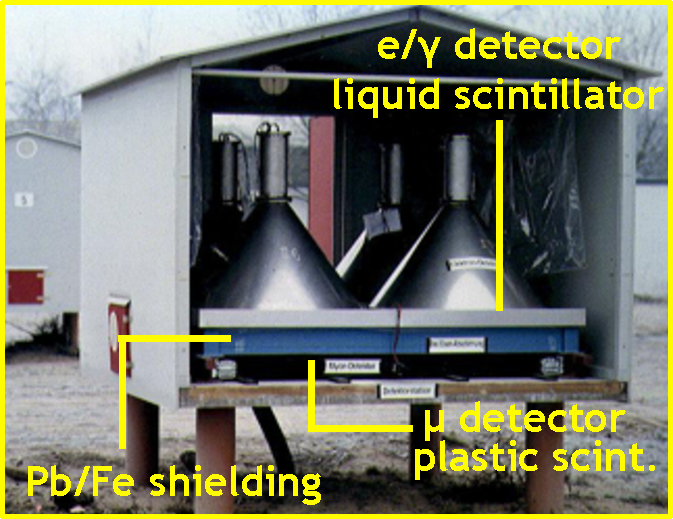
\includegraphics[width=1\textwidth]{pics/KASCADE-station.pdf}
\end{minipage}
\end{frame}

\begin{frame}{KASCADE-Grande $\gamma$ ray searches}
\begin{itemize}
 \item Limits on the diffuse gamma-ray flux: the best upper limit of the fraction of $\gamma$-rays
to the total cosmic ray flux is obtained at $3.7 \times 10^{15}$~eV and equals $1.1 \times 10^{-5}$.
\end{itemize}
\begin{center}
  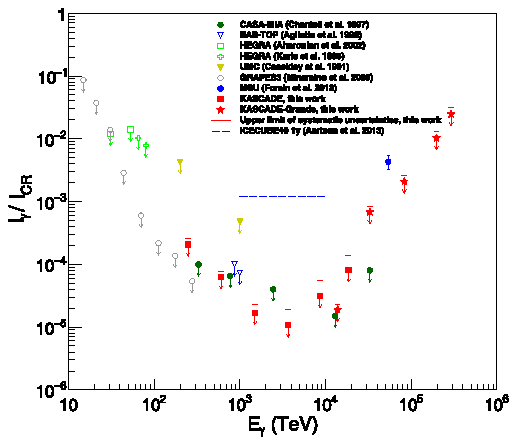
\includegraphics[height=0.56\textheight]{pics/KASCADE-Grande_UHECR2016-1.pdf}
  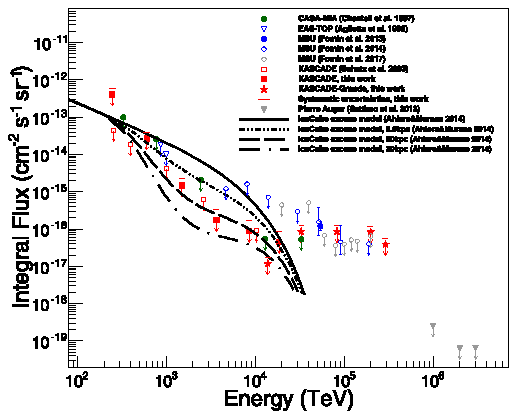
\includegraphics[height=0.56\textheight]{pics/KASCADE-Grande_UHECR2016-2.pdf}
\end{center}
\vspace{-2ex}
\small
[1] W.~Apel et al., \textit{KASCADE-Grande Limits on the Isotropic Diffuse Gamma-Ray Flux between 100~TeV and 1~EeV}, 2017, ApJ, 848, 1.
\end{frame}
